\documentclass[12pt]{article}

\usepackage[margin = .8in]{geometry}
\usepackage{amsmath}
\usepackage{graphicx}
\usepackage{multicol, enumitem, adjustbox}

\usepackage{fancyhdr}
\pagestyle{fancy}

\lhead{Math F113X: Numbers and Society}
\rhead{}

\usepackage{tikz}
\usetikzlibrary{calc,trees,positioning,arrows,fit,shapes,calc}
\usetikzlibrary{patterns}
\usepackage{pgfplots}

\usepackage{longtable}
\usepackage{tabularx}

\newcommand{\ds}{\displaystyle}
\newcommand{\ans}[1][1in]{\rule{#1}{.5pt}}

\newcommand{\points}[1]{(#1 points.)}		% Trying to be lazy.

\usepackage{array}
\newcolumntype{L}[1]{>{\raggedright\let\newline\\\arraybackslash\hspace{0pt}}m{#1}}
\newcolumntype{C}[1]{>{\centering\let\newline\\\arraybackslash\hspace{0pt}}m{#1}}
\newcolumntype{R}[1]{>{\raggedleft\let\newline\\\arraybackslash\hspace{0pt}}m{#1}}
\newcommand{\red}[1]{\textcolor{red}{#1}}

%\topmargin -1in
%\textheight 9.5in
%\oddsidemargin -0.3in
%\evensidemargin \oddsidemargin
%\pagestyle{empty}
%%\marginparwidth 0.5in
%\textwidth 7in
%\parindent 0in

%--------------------------------------------------------------------------------------------------------------------------------------------------------------------------
%						Document
%--------------------------------------------------------------------------------------------------------------------------------------------------------------------------


\begin{document}
%\pagestyle{fancy}
\begin{center}
{\Large  Worksheet 6:  Fair Shares and Divider-Chooser 	}
\end{center}



%\noindent \textbf{Group Names:} \hrulefill \\
%-------------------------------------------------------------------------------------------------------------
%						Assignment
%-----------------------------------------------------------------------------------------------------


%\begin{minipage}[b]{.6\linewidth}
Tom and Fred were given a cake worth \$12 that is equal parts strawberry, vanilla and chocolate.% Tom likes vanilla and strawberry the same but does not like chocolate at all. Fred will eat vanilla but likes strawberry twice as much as vanilla and likes chocolate three times as much as vanilla.

%\end{minipage}

\begin{center}
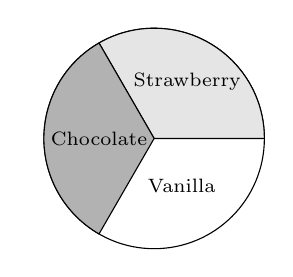
\begin{tikzpicture}[scale=0.7]
\def\r{2}
\draw (0,0) circle (\r cm);
\filldraw[fill= gray!20 ] (0,0) -- (0:\r) arc (0:120:\r) -- (0,0);
\path (60:1.2) node[]{{{\scriptsize Strawberry}}};
%\path node[right] (240:1) {{\scriptsize Strawberry}};
\filldraw[fill = gray!60 ] (0,0) -- (120:\r) arc (120:240:\r) -- (0,0);
\path (120+60:\r/2) node[]{{{\scriptsize Chocolate}}};
\path (-60:\r/2) node[]{{{\scriptsize Vanilla}}};
\end{tikzpicture}
\end{center}

%
%\begin{minipage}[b]{.4\linewidth}

%\end{minipage}

\begin{enumerate}
\item How much value is a fair share of the cake? \ans

\item Tom likes vanilla and strawberry equally, and doesn't like chocolate at all. Label the cake parts as you answer the following:


\begin{minipage}{.6\textwidth}
    \begin{itemize}
    \item How much does Tom value the vanilla section of the cake? \ans
    \item How much does Tom value the chocolate section of the cake? \ans
    \item How much does Tom value the strawberry section of the cake? \ans
    \item Find (and draw) two \emph{different} ways Tom could split the cake into two pieces of equal value.
    \end{itemize}
    \end{minipage}
\begin{minipage}{.3\textwidth}
\hfill
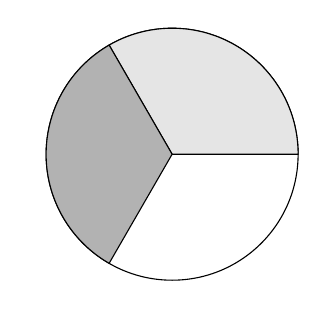
\begin{tikzpicture}[scale=0.8]
\draw (0,0) circle (2 cm);
\filldraw[fill= gray!20 ] (0,0) -- (0:2) arc (0:120:2) -- (0,0);
\filldraw[fill = gray!60 ] (0,0) -- (120:2) arc (120:240:2) -- (0,0);
\end{tikzpicture}
\hfill
\hfill 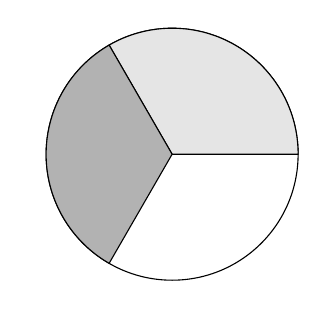
\begin{tikzpicture}[scale=0.8]
\draw (0,0) circle (2 cm);
\filldraw[fill= gray!20 ] (0,0) -- (0:2) arc (0:120:2) -- (0,0);
\filldraw[fill = gray!60 ] (0,0) -- (120:2) arc (120:240:2) -- (0,0);
\end{tikzpicture}
\end{minipage}
\vfill

\item Fred will eat vanilla, but he likes strawberry twice as much as vanilla and he likes chocolate \emph{three} times as much as vanilla. Label the cake parts.

\begin{minipage}{.6\textwidth}
\begin{itemize}
\item How much does Fred value the vanilla section of the cake? \ans
\item How much does Fred value the chocolate section of the cake? \ans
\item How much does Fred value the strawberry section of the cake? \ans
\item Find (and draw) two \emph{different} ways Tom could split the cake into two pieces of equal value.
\end{itemize}
\end{minipage}
\begin{minipage}{.3\textwidth}
\hfill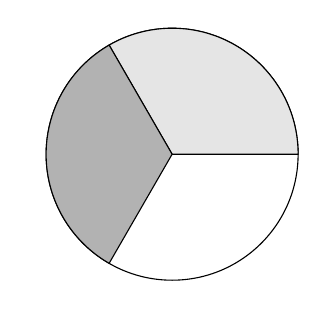
\begin{tikzpicture}[scale=0.8]
\draw (0,0) circle (2 cm);
\filldraw[fill= gray!20 ] (0,0) -- (0:2) arc (0:120:2) -- (0,0);
\filldraw[fill = gray!60 ] (0,0) -- (120:2) arc (120:240:2) -- (0,0);
\end{tikzpicture}
\hfill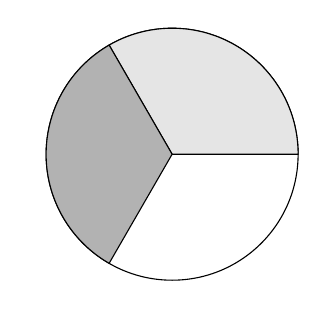
\begin{tikzpicture}[scale=0.8]
\draw (0,0) circle (2 cm);
\filldraw[fill= gray!20 ] (0,0) -- (0:2) arc (0:120:2) -- (0,0);
\filldraw[fill = gray!60 ] (0,0) -- (120:2) arc (120:240:2) -- (0,0);
\end{tikzpicture}
\end{minipage}

\vfill

\newpage

You are going to demonstrate how to divide the cake between Tom and Fred using the Divider-Chooser Method.\\ 
Steps: \\
(1) Divide the cake into two pieces of equal value according to the \textbf{Divider's} values. (Label these two pieces in both pictures).\\
(2) Determine which piece the \textbf{Chooser} will select according to their values. \\
(3) Assign the remaining piece to the \textbf{Divider}.\\
(4) Calculate the value of the final outcome for each person.

\item \textbf{Divider:} Tom; \quad \textbf{Chooser:} Fred. 
\def\r{1.2}

\begin{tikzpicture}
\draw (0,0) circle (\r cm);
\filldraw[fill= gray!20 ] (0,0) -- (0:\r) arc (0:120:\r) -- (0,0);
\filldraw[fill = gray!60 ] (0,0) -- (120:\r) arc (120:240:\r) -- (0,0);
\node at (60: \r/2){\$6};
\node at (-60: \r/2){\$6};
\node at (180: \r/2){\$0};
\path (90:\r) node [above] {Tom's Values};
\end{tikzpicture}\hspace{2cm}\begin{tikzpicture}
\draw (0,0) circle (\r cm);
\filldraw[fill= gray!20 ] (0,0) -- (0:\r) arc (0:120:\r) -- (0,0);
\filldraw[fill = gray!60 ] (0,0) -- (120:\r) arc (120:240:\r) -- (0,0);
\node at (60: \r/2){\$4};
\node at (-60: \r/2){\$2};
\node at (180: \r/2){\$6};
\path (90:\r) node [above] {Fred's Values};
\end{tikzpicture}
\hfill
\begin{tabular}{c|c|c}
\multicolumn{3}{c}{\textbf{Final Outcome}}\\
\hline \hline
&\quad Tom \quad &\quad  Fred \quad \\
\hline
&&\\
share&&\\
\hline
&&\\
value&&\\
\end{tabular}
\vfill


\vspace{1cm}

\item  \textbf{Chooser:} Tom \quad \textbf{Divider:} Fred; \quad 
\def\r{1.2}

\begin{tikzpicture}
\draw (0,0) circle (\r cm);
\filldraw[fill= gray!20 ] (0,0) -- (0:\r) arc (0:120:\r) -- (0,0);
\filldraw[fill = gray!60 ] (0,0) -- (120:\r) arc (120:240:\r) -- (0,0);
\node at (60: \r/2){\$6};
\node at (-60: \r/2){\$6};
\node at (180: \r/2){\$0};
\path (90:\r) node [above] {Tom's Values};
\end{tikzpicture}\hspace{2cm}\begin{tikzpicture}
\draw (0,0) circle (\r cm);
\filldraw[fill= gray!20 ] (0,0) -- (0:\r) arc (0:120:\r) -- (0,0);
\filldraw[fill = gray!60 ] (0,0) -- (120:\r) arc (120:240:\r) -- (0,0);
\node at (60: \r/2){\$4};
\node at (-60: \r/2){\$2};
\node at (180: \r/2){\$6};
\path (90:\r) node [above] {Fred's Values};
\end{tikzpicture}
\hfill
\begin{tabular}{c|c|c}
\multicolumn{3}{c}{\textbf{Final Outcome}}\\
\hline \hline
& \quad Tom \quad &\quad  Fred\quad \\
\hline
&&\\
share&&\\
\hline
&&\\
value&&\\
\end{tabular}
\vfill


\vspace{1cm}


%\item Find two different ways for Fred to divide the cake into two shares (not necessarily connected) that he values equally. In each case, which share should Tom choose to make sure he gets his fair share?
%
%\begin{tikzpicture}
%\draw (0,0) circle (\r cm);
%\filldraw[fill= gray!20 ] (0,0) -- (0:\r) arc (0:120:\r) -- (0,0);
%\filldraw[fill = gray!60 ] (0,0) -- (120:\r) arc (120:240:\r) -- (0,0);
%\path (90:\r) node [above] {Tom's Values};
%\end{tikzpicture}\hspace{2cm}\begin{tikzpicture}
%\draw (0,0) circle (\r cm);
%\filldraw[fill= gray!20 ] (0,0) -- (0:\r) arc (0:120:\r) -- (0,0);
%\filldraw[fill = gray!60 ] (0,0) -- (120:\r) arc (120:240:\r) -- (0,0);
%\path (90:\r) node [above] {Fred's Values};
%\end{tikzpicture}
%\vfill
%
%\begin{tikzpicture}
%\draw (0,0) circle (\r cm);
%\filldraw[fill= gray!20 ] (0,0) -- (0:\r) arc (0:120:\r) -- (0,0);
%\filldraw[fill = gray!60 ] (0,0) -- (120:\r) arc (120:240:\r) -- (0,0);
%\path (90:\r) node [above] {Tom's Values};
%\end{tikzpicture}\hspace{2cm}\begin{tikzpicture}
%\draw (0,0) circle (\r cm);
%\filldraw[fill= gray!20 ] (0,0) -- (0:\r) arc (0:120:\r) -- (0,0);
%\filldraw[fill = gray!60 ] (0,0) -- (120:\r) arc (120:240:\r) -- (0,0);
%\path (90:\r) node [above] {Fred's Values};
%\end{tikzpicture}
%\vfill

\item Is it better to be the divider or chooser in this case? Why? 

\vspace{1cm}

\begin{minipage}{.7\textwidth}
\item Challenge: Suppose that another friend, Janet, likes vanilla 3 times as much as she likes strawberry and chocolate, which she likes equally. How much does she value each of the three pieces?
\end{minipage}
\begin{minipage}{.3\textwidth}
%\vspace{1.5in}
\hfill\begin{tikzpicture}
\draw (0,0) circle (\r cm);
\filldraw[fill= gray!20 ] (0,0) -- (0:\r) arc (0:120:\r) -- (0,0);
\filldraw[fill = gray!60 ] (0,0) -- (120:\r) arc (120:240:\r) -- (0,0);
\path (90:\r) node [above] {Janet's Values};
\end{tikzpicture}
\end{minipage}

Strawberry \ans Vanilla \ans Chocolate \ans

\end{enumerate}

\end{document}

%-------------------------------------------------------------------------------------------------------------------------------------------------------------------------------------------------------------------

%%% Local Variables:
%%% mode: latex
%%% TeX-master: t
%%% End:
